% Niveau :      PC
% Discipline :  Mécaflu
%Mots clés :    Viscosité, Couche limite, Equation de Blasius

\begin{exercise}{Couche limite visqueuse de Blasius}{3}{Spé}
{Mécanique des fluides, Fluides réels}{bermu}

\begin{questions}
    \questioncours Décrire les différents termes de l'équation de Navier--Stockes en 2D et définir le nombre de Reynolds $\ReN$. On prendra soin de la garder dans un coin du tableau pour la suite. \\
    Définir ce qu'est la \emph{couche limite} $\delta$ d'un écoulement et en donner un critère qualitatif.
\begin{EnvUplevel}
Nous étudions par la suite l'évolution du profil 2D de vitesse $\mqty(u_x \\ u_y)$ pour un écoulement de couche limite au-dessus d'une plaque plane :
\begin{figure}[H]
    \centering
    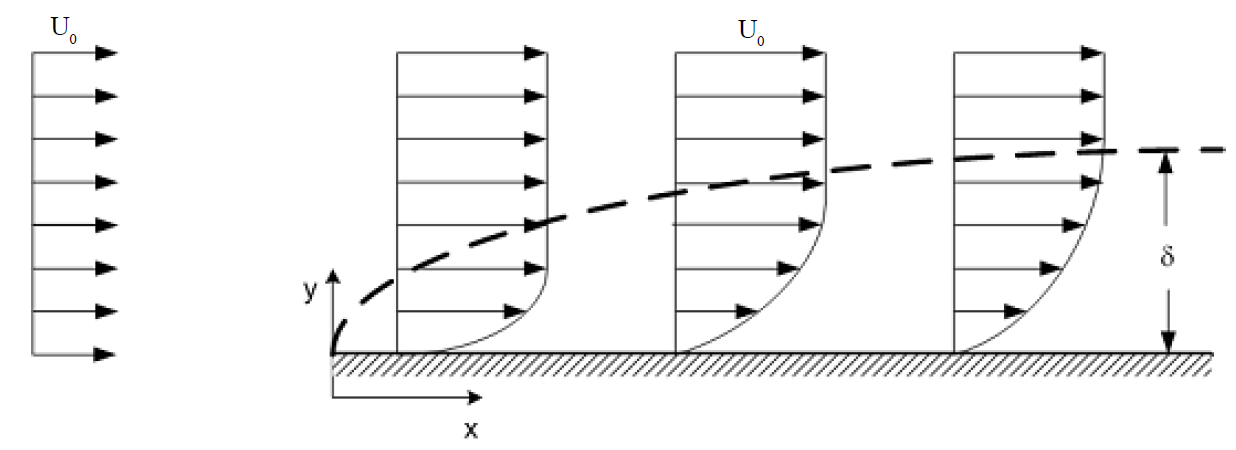
\includegraphics[width=0.8\linewidth]{mecaflu/blasius1.png}
    \vspace{-1em}
    \caption{Schéma du profil de couche limite au-dessus d'une plaque plane.}
\end{figure}
Dans ce cas, la taille de la couche limite $\delta(x)$ varie selon la distance $x$ parcourue le long de la plaque plane par le fluide.
\end{EnvUplevel}
    \question En vous aidant du schéma ci-dessus, donner les conditions aux limites pour la vitesse $u_x$, $u_y$ et la pression $p$.
\uplevel{Nous introduisons $\ReN_x$, le nombre de Reynolds ayant pour taille caractéristique $x$. Nous considérerons que la couche étudiée limite est visqueuse (par opposition à turbulente).}
    \question Quelle est l'expression de $\ReN_x$ ? Quel est son sens physique ? Est-il grand ou petit ?
    \question Justifier qualitativement que pour $y\gg\delta(x)$, les effets de viscosité sont négligeables et que par conséquent la pression y est constante $p(x,y) \simeq p_0$.
    \question Inversement, justifier qualitativement que pour $y\ll\delta(x)$, une variation de hauteur typique $\delta(x)$ peut s'écrire
    $$\delta(x) \simeq \sqrt{\dfrac{\nu x}{U_0}}.$$
    \question En utilisant le nombre de Reynolds $\ReN_x$ et le résultat précédent, justifier que
    $$\pdv{}{y} \ll \pdv{}{x},$$
    et en déduire que
    \begin{parts}
        \part la pression $p$ dans la couche limite est égale à la pression au-dessus de la couche limite ;
        \part la vitesse verticale $u_y$ ne peut pas être nulle dans la couche limite.
    \end{parts}
    \question Utilisez les résultats précédents simplifier l'équation de Navier--Stockes suivant $x$. \\
    L'équation ne comportera plus que trois termes.
    \questionbonus Cette équation peut être généralisée à n'importe quel profil d'attaque : reprendre la question précédente en prenant en compte que cette fois-ci $U_0(x)$ dépend de $x$.
\end{questions}

\begin{center}
    \itshape --- \quad Suite au verso \quad ---
\end{center}
\end{exercise}
\pagebreak

\printexerciseheader

\begin{center}
    \itshape --- \quad Suite du recto \quad ---
\end{center}

\bigskip

\begin{questions}
\setcounter{question}{8}
\question En justifiant succinctement et en utilisant le changement de variable suivant :
    $$u_x = U_0 f'(\xi), \qquad y = \xi\delta(x),$$
    montrez que l'équation de Navier--Stockes et l'équation d'incompressibilité permettent de d'obtenir l'équation de Blasius
    $$2 f'''(\xi) + f(\xi) f''(\xi) = 0.$$
    
    \textbf{Aide :} les dérivées partielles s'écrivent dans ce cas
    $$\pdv{}{x} = -\dfrac{\xi}{2x}\pdv{}{\xi} \qqtext{et} \pdv{}{y} = \dfrac{1}{\delta(x)}\pdv{}{\xi}.$$
\uplevel{L'équation de Blasius est non linéaire et ne peut être obtenue que par intégration numérique. Il faut donc trouver des conditions aux limites pour $f$.}
    \question Justifier que celles employées pour la figure ci-dessous sont
    $$f'(0) = 0,\quad f'(\infty) = 1, \quad f'''(0) = 0.$$
\begin{EnvUplevel}
La solution numérique est alors :
\begin{figure}[H]
    \centering
    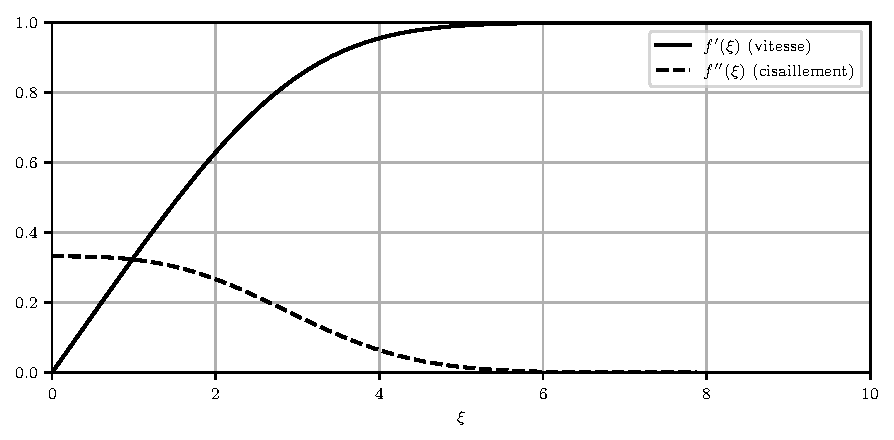
\includegraphics[scale=1]{mecaflu/blasius2.pdf}
    \vspace{-1em}
    \caption{Solution de l'équation de Blasius.}
\end{figure}
\end{EnvUplevel}
    \question En déduire un critère plus rigoureux pour l'épaisseur de la couche limite.
\end{questions}

\plusloin
Décrire qualitativement l'écoulement pour $x \gg \dfrac{\nu}{U_0}$ et faire un schéma représentant les deux régimes.

\newpage